\section{The Explicit-Control Evaluator}
\label{Section 5.4}

In \cref{Section 5.1} we saw how to transform simple Scheme programs into descriptions of register machines.
We will now perform this transformation on a more complex program, the metacircular evaluator of \cref{Section 4.1.1}--\cref{Section 4.1.4}, which shows how the behavior of a Scheme interpreter can be described in terms of the procedures \code{eval} and \code{apply}.
The \newterm{explicit-control evaluator} that we develop in this section shows how the underlying procedure-calling and argument-passing mechanisms used in the evaluation process can be described in terms of operations on registers and stacks.
In addition, the explicit-control evaluator can serve as an implementation of a Scheme interpreter, written in a language that is very similar to the native machine language of conventional computers.
The evaluator can be executed by the register-machine simulator of \cref{Section 5.2}.
Alternatively, it can be used as a starting point for building a machine-language implementation of a Scheme evaluator, or even a special-purpose machine for evaluating Scheme expressions.
\cref{Figure 5.16} shows such a hardware implementation:
a silicon chip that acts as an evaluator for Scheme.
The chip designers started with the data-path and controller specifications for a register machine similar to the evaluator described in this section and used design automation programs to construct the integrated-circuit layout.%
\footnote{
	See \cref{Batali et al. 1982} for more information on the chip and the method by which it was designed.
}

\begin{figure}[tb]
	\centering
	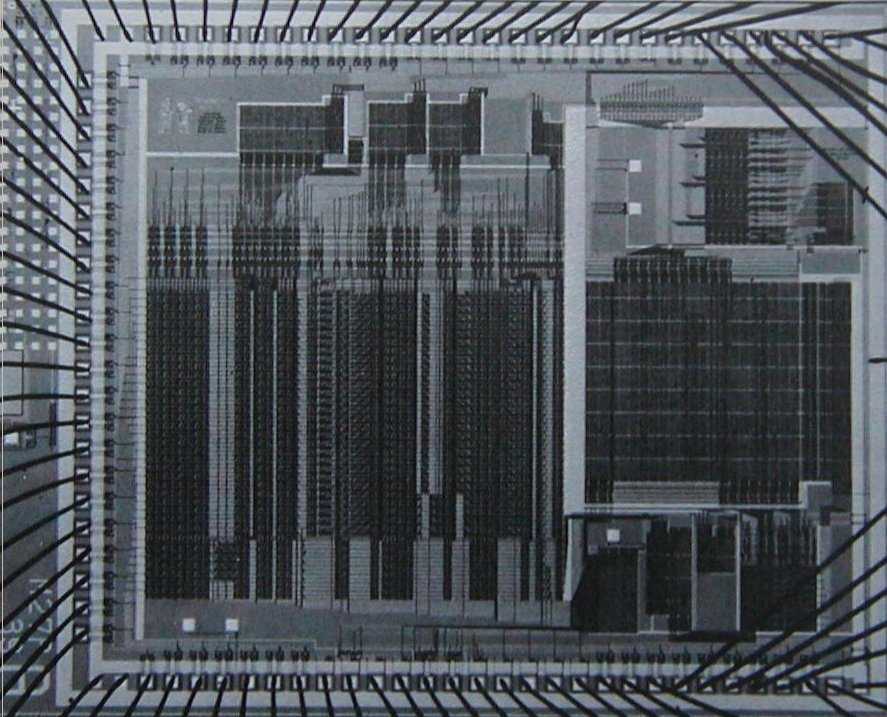
\includegraphics[width=91mm]{fig/chap5/chip.jpg}
	\caption{
		A silicon-chip implementation of an evaluator for Scheme.
	}
	\label{Figure 5.16}
\end{figure}



\subsubsection*{Registers and operations}

In designing the explicit-control evaluator, we must specify the operations to be used in our register machine.
We described the metacircular evaluator in terms of abstract syntax, using procedures such as \code{quoted?} and \code{make-procedure}.
In implementing the register machine, we could expand these procedures into sequences of elementary list-structure memory operations, and implement these operations on our register machine.
However, this would make our evaluator very long, obscuring the basic structure with details.
To clarify the presentation, we will include as primitive operations of the register machine the syntax procedures given in \cref{Section 4.1.2} and the procedures for representing environments and other run-time data given in sections \cref{Section 4.1.3} and \cref{Section 4.1.4}.
In order to completely specify an evaluator that could be programmed in a low-level machine language or implemented in hardware, we would replace these operations by more elementary operations, using the list-structure implementation we described in \cref{Section 5.3}.

Our Scheme evaluator register machine includes a stack and seven registers:
\code{exp}, \code{env}, \code{val}, \code{continue}, \code{proc}, \code{argl}, and \code{unev}.
\code{exp} is used to hold the expression to be evaluated, and \code{env} contains the environment in which the evaluation is to be performed.
At the end of an evaluation, \code{val} contains the value obtained by evaluating the expression in the designated environment.
The \code{continue} register is used to implement recursion, as explained in \cref{Section 5.1.4}.
(The evaluator needs to call itself recursively, since evaluating an expression requires evaluating its subexpressions.)
The registers \code{proc}, \code{argl}, and \code{unev} are used in evaluating combinations.

We will not provide a data-path diagram to show how the registers and operations of the evaluator are connected, nor will we give the complete list of machine operations.
These are implicit in the evaluator’s controller, which will be presented in detail.

\subsection{The Core of the Explicit-Control Evaluator}
\label{Section 5.4.1}

The central element in the evaluator is the sequence of instructions beginning at \code{eval-dispatch}.
This corresponds to the \code{eval} procedure of the metacircular evaluator described in \cref{Section 4.1.1}.
When the controller starts at \code{eval-dispatch}, it evaluates the expression specified by \code{exp} in the environment specified by \code{env}.
When evaluation is complete, the controller will go to the entry point stored in \code{continue}, and the \code{val} register will hold the value of the expression.
As with the metacircular \code{eval}, the structure of \code{eval-dispatch} is a case analysis on the syntactic type of the expression to be evaluated.%
\footnote{
	In our controller, the dispatch is written as a sequence of \code{test} and \code{branch} instructions.
	Alternatively, it could have been written in a data-directed style (and in a real system it probably would have been) to avoid the need to perform sequential tests and to facilitate the definition of new expression types.
	A machine designed to run Lisp would probably include a \code{dispatch-on-type} instruction that would efficiently execute such data-directed dispatches.
}

\begin{scheme}
  eval-dispatch
    (test (op self-evaluating?) (reg exp))
    (branch (label ev-self-eval))
    (test (op variable?) (reg exp))
    (branch (label ev-variable))
    (test (op quoted?) (reg exp))
    (branch (label ev-quoted))
    (test (op assignment?) (reg exp))
    (branch (label ev-assignment))
    (test (op definition?) (reg exp))
    (branch (label ev-definition))
    (test (op if?) (reg exp))
    (branch (label ev-if))
    (test (op lambda?) (reg exp))
    (branch (label ev-lambda))
    (test (op begin?) (reg exp))
    (branch (label ev-begin))
    (test (op application?) (reg exp))
    (branch (label ev-application))
    (goto (label unknown-expression-type))
\end{scheme}



\subsubsection*{Evaluating simple expressions}

Numbers and strings (which are self-evaluating), variables, quotations, and \code{lambda} expressions have no subexpressions to be evaluated.
For these, the evaluator simply places the correct value in the \code{val} register and continues execution at the entry point specified by \code{continue}.
Evaluation of simple expressions is performed by the following controller code:
\begin{scheme}
  ev-self-eval
    (assign val (reg exp))
    (goto (reg continue))
  ev-variable
    (assign val (op lookup-variable-value) (reg exp) (reg env))
    (goto (reg continue))
  ev-quoted
    (assign val (op text-of-quotation) (reg exp))
    (goto (reg continue))
  ev-lambda
    (assign unev (op lambda-parameters) (reg exp))
    (assign exp (op lambda-body) (reg exp))
    (assign val (op make-procedure) (reg unev) (reg exp) (reg env))
    (goto (reg continue))
\end{scheme}
Observe how \code{ev-lambda} uses the \code{unev} and \code{exp} registers to hold the parameters and body of the lambda expression so that they can be passed to the \code{make-procedure} operation, along with the environment in \code{env}.



\subsubsection*{Evaluating procedure applications}

A procedure application is specified by a combination containing an operator and operands.
The operator is a subexpression whose value is a procedure, and the operands are subexpressions whose values are the arguments to which the procedure should be applied.
The metacircular \code{eval} handles applications by calling itself recursively to evaluate each element of the combination, and then passing the results to \code{apply}, which performs the actual procedure application.
The explicit-control evaluator does the same thing;
these recursive calls are implemented by \code{goto} instructions, together with use of the stack to save registers that will be restored after the recursive call returns.
Before each call we will be careful to identify which registers must be saved (because their values will be needed later).%
\footnote{
	This is an important but subtle point in translating algorithms from a procedural language, such as Lisp, to a register-machine language.
	As an alternative to saving only what is needed, we could save all the registers (except \code{val}) before each recursive call.
	This is called a \newterm{framed-stack} discipline.
	This would work but might save more registers than necessary;
	this could be an important consideration in a system where stack operations are expensive.
	Saving registers whose contents will not be needed later may also hold onto useless data that could otherwise be garbage-collected, freeing space to be reused.
}

We begin the evaluation of an application by evaluating the operator to produce a procedure, which will later be applied to the evaluated operands.
To evaluate the operator, we move it to the \code{exp} register and go to \code{eval-dispatch}.
The environment in the \code{env} register is already the correct one in which to evaluate the operator.
However, we save \code{env} because we will need it later to evaluate the operands.
We also extract the operands into \code{unev} and save this on the stack.
We set up \code{continue} so that \code{eval-dispatch} will resume at \code{ev-appl-did-operator} after the operator has been evaluated.
First, however, we save the old value of \code{continue}, which tells the controller where to continue after the application.

\begin{scheme}
  ev-application
    (save continue)
    (save env)
    (assign unev (op operands) (reg exp))
    (save unev)
    (assign exp (op operator) (reg exp))
    (assign continue (label ev-appl-did-operator))
    (goto (label eval-dispatch))
\end{scheme}

Upon returning from evaluating the operator subexpression, we proceed to evaluate the operands of the combination and to accumulate the resulting arguments in a list, held in \code{argl}.
First we restore the unevaluated operands and the environment.
We initialize \code{argl} to an empty list.
Then we assign to the \code{proc} register the procedure that was produced by evaluating the operator.
If there are no operands, we go directly to \code{apply-dispatch}.
Otherwise we save \code{proc} on the stack and start the argument-evaluation loop:%
\footnote{
	We add to the evaluator data-structure procedures in \cref{Section 4.1.3} the following two procedures for manipulating argument lists:
	\begin{smallscheme}
	  (define (empty-arglist) '())
	  (define (adjoin-arg arg arglist) (append arglist (list arg)))
	\end{smallscheme}
	We also use an additional syntax procedure to test for the last operand in a combination:
	\begin{smallscheme}
	  (define (last-operand? ops) (null? (cdr ops)))
	\end{smallscheme}
}
\begin{scheme}
  ev-appl-did-operator
    (restore unev)                       ~\textrm{; the operands}~
    (restore env)
    (assign argl (op empty-arglist))
    (assign proc (reg val))              ~\textrm{; the operator}~
    (test (op no-operands?) (reg unev))
    (branch (label apply-dispatch))
    (save proc)
\end{scheme}

Each cycle of the argument-evaluation loop evaluates an operand from the list in \code{unev} and accumulates the result into \code{argl}.
To evaluate an operand, we place it in the \code{exp} register and go to \code{eval-dispatch}, after setting \code{continue} so that execution will resume with the argument-accumulation phase.
But first we save the arguments accumulated so far (held in \code{argl}), the environment (held in \code{env}), and the remaining operands to be evaluated (held in \code{unev}).
A special case is made for the evaluation of the last operand, which is handled at \code{ev-appl-last-arg}.

\begin{scheme}
  ev-appl-operand-loop
    (save argl)
    (assign exp (op first-operand) (reg unev))
    (test (op last-operand?) (reg unev))
    (branch (label ev-appl-last-arg))
    (save env)
    (save unev)
    (assign continue (label ev-appl-accumulate-arg))
    (goto (label eval-dispatch))
\end{scheme}

When an operand has been evaluated, the value is accumulated into the list held in \code{argl}.
The operand is then removed from the list of unevaluated operands in \code{unev}, and the argument-evaluation continues.

\begin{scheme}
  ev-appl-accumulate-arg
    (restore unev)
    (restore env)
    (restore argl)
    (assign argl (op adjoin-arg) (reg val) (reg argl))
    (assign unev (op rest-operands) (reg unev))
    (goto (label ev-appl-operand-loop))
\end{scheme}

Evaluation of the last argument is handled differently.
There is no need to save the environment or the list of unevaluated operands before going to \code{eval-dispatch}, since they will not be required after the last operand is evaluated.
Thus, we return from the evaluation to a special entry point \code{ev-appl-accum-last-arg}, which restores the argument list, accumulates the new argument, restores the saved procedure, and goes off to perform the application.%
\footnote{
	The optimization of treating the last operand specially is known as \newterm{evlis tail recursion} (see \cref{Wand 1980}).
	We could be somewhat more efficient in the argument evaluation loop if we made evaluation of the first operand a special case too.
	This would permit us to postpone initializing \code{argl} until after evaluating the first operand, so as to avoid saving \code{argl} in this case.
	The compiler in \cref{Section 5.5} performs this optimization.
	(Compare the \code{construct-arglist} procedure of \cref{Section 5.5.3}.)
}

\begin{scheme}
  ev-appl-last-arg
    (assign continue (label ev-appl-accum-last-arg))
    (goto (label eval-dispatch))
  ev-appl-accum-last-arg
    (restore argl)
    (assign argl (op adjoin-arg) (reg val) (reg argl))
    (restore proc)
    (goto (label apply-dispatch))
\end{scheme}

The details of the argument-evaluation loop determine the order in which the interpreter evaluates the operands of a combination (e.g., left to right or right to left---see \cref{Exercise 3.8}).
This order is not determined by the metacircular evaluator, which inherits its control structure from the underlying Scheme in which it is implemented.%
\footnote{
	The order of operand evaluation in the metacircular evaluator is determined by the order of evaluation of the arguments to \code{cons} in the procedure \code{list-of-values} of \cref{Section 4.1.1} (see \cref{Exercise 4.1}).
}
	Because the \code{first-operand} selector (used in \code{ev-appl-operand-loop} to extract successive operands from \code{unev}) is implemented as \code{car} and the \code{rest-operands} selector is implemented as \code{cdr}, the explicit-control evaluator will evaluate the operands of a combination in left-to-right order.



\subsubsection*{Procedure application}

The entry point \code{apply-dispatch} corresponds to the \code{apply} procedure of the metacircular evaluator.
By the time we get to \code{apply-dispatch}, the \code{proc} register contains the procedure to apply and \code{argl} contains the list of evaluated arguments to which it must be applied.
The saved value of \code{continue} (originally passed to \code{eval-dispatch} and saved at \code{ev-application}), which tells where to return with the result of the procedure application, is on the stack.
When the application is complete, the controller transfers to the entry point specified by the saved \code{continue}, with the result of the application in \code{val}.
As with the metacircular \code{apply}, there are two cases to consider.
Either the procedure to be applied is a primitive or it is a compound procedure.

\begin{scheme}
  apply-dispatch
  (test (op primitive-procedure?) (reg proc))
  (branch (label primitive-apply))
  (test (op compound-procedure?) (reg proc))
  (branch (label compound-apply))
  (goto (label unknown-procedure-type))
\end{scheme}

We assume that each primitive is implemented so as to obtain its arguments from \code{argl} and place its result in \code{val}.
To specify how the machine handles primitives, we would have to provide a sequence of controller instructions to implement each primitive and arrange for \code{primitive-apply} to dispatch to the instructions for the primitive identified by the contents of \code{proc}.
Since we are interested in the structure of the evaluation process rather than the details of the primitives, we will instead just use an \code{apply-primitive-procedure} operation that applies the procedure in \code{proc} to the arguments in \code{argl}.
For the purpose of simulating the evaluator with the simulator of \cref{Section 5.2} we use the procedure \code{apply-primitive-procedure}, which calls on the underlying Scheme system to perform the application, just as we did for the metacircular evaluator in \cref{Section 4.1.4}.
After computing the value of the primitive application, we restore \code{continue} and go to the designated entry point.

\begin{scheme}
  primitive-apply
    (assign val (op apply-primitive-procedure)
                (reg proc)
              (reg argl))
  (restore continue)
  (goto (reg continue))
\end{scheme}

To apply a compound procedure, we proceed just as with the metacircular evaluator.
We construct a frame that binds the procedure’s parameters to the arguments, use this frame to extend the environment carried by the procedure, and evaluate in this extended environment the sequence of expressions that forms the body of the procedure.
\code{ev-sequence}, described below in \cref{Section 5.4.2}, handles the evaluation of the sequence.

\begin{scheme}
  compound-apply
    (assign unev (op procedure-parameters) (reg proc))
    (assign env (op procedure-environment) (reg proc))
    (assign env (op extend-environment)
                (reg unev) (reg argl) (reg env))
    (assign unev (op procedure-body) (reg proc))
    (goto (label ev-sequence))
\end{scheme}

\code{compound-apply} is the only place in the interpreter where the \code{env} register is ever assigned a new value.
Just as in the metacircular evaluator, the new environment is constructed from the environment carried by the procedure, together with the argument list and the corresponding list of variables to be bound.

\subsection{Sequence Evaluation and Tail Recursion}
\label{Section 5.4.2}

The portion of the explicit-control evaluator at \code{ev-sequence} is analogous to the metacircular evaluator’s \code{eval-sequence} procedure.
It handles sequences of expressions in procedure bodies or in explicit \code{begin} expressions.

Explicit \code{begin} expressions are evaluated by placing the sequence of expressions to be evaluated in \code{unev}, saving \code{continue} on the stack, and jumping to \code{ev-sequence}.
\begin{scheme}
  ev-begin
    (assign unev (op begin-actions) (reg exp))
    (save continue)
    (goto (label ev-sequence))
\end{scheme}
The implicit sequences in procedure bodies are handled by jumping to
\code{ev-sequence} from \code{compound-apply}, at which point \code{continue}
is already on the stack, having been saved at \code{ev-application}.

The entries at \code{ev-sequence} and \code{ev-sequence-continue} form a loop that successively evaluates each expression in a sequence.
The list of unevaluated expressions is kept in \code{unev}.
Before evaluating each expression, we check to see if there are additional expressions to be evaluated in the sequence.
If so, we save the rest of the unevaluated expressions (held in \code{unev}) and the environment in which these must be evaluated (held in \code{env}) and call \code{eval-dispatch} to evaluate the expression.
The two saved registers are restored upon the return from this evaluation, at \code{ev-sequence-continue}.

The final expression in the sequence is handled differently, at the entry point \code{ev-sequence-last-exp}.
Since there are no more expressions to be evaluated after this one, we need not save \code{unev} or \code{env} before going to \code{eval-dispatch}.
The value of the whole sequence is the value of the last expression, so after the evaluation of the last expression there is nothing left to do except continue at the entry point currently held on the stack (which was saved by \code{ev-application} or \code{ev-begin}.)
Rather than setting up \code{continue} to arrange for \code{eval-dispatch} to return here and then restoring \code{continue} from the stack and continuing at that entry point, we restore \code{continue} from the stack before going to \code{eval-dispatch}, so that \code{eval-dispatch} will continue at that entry point after evaluating the expression.

\begin{scheme}
  ev-sequence
    (assign exp (op first-exp) (reg unev))
    (test (op last-exp?) (reg unev))
    (branch (label ev-sequence-last-exp))
    (save unev)
    (save env)
    (assign continue (label ev-sequence-continue))
    (goto (label eval-dispatch))
  ev-sequence-continue
    (restore env)
    (restore unev)
    (assign unev (op rest-exps) (reg unev))
    (goto (label ev-sequence))
  ev-sequence-last-exp
    (restore continue)
    (goto (label eval-dispatch))
\end{scheme}



\subsubsection*{Tail recursion}

In \link{Chapter 1} we said that the process described by a procedure such as
\begin{scheme}
  (define (sqrt-iter guess x)
    (if (good-enough? guess x)
        guess
        (sqrt-iter (improve guess x) x)))
\end{scheme}
is an iterative process.
Even though the procedure is syntactically recursive (defined in terms of itself), it is not logically necessary for an evaluator to save information in passing from one call to \code{sqrt-iter} to the next.%
\footnote{
	We saw in \link{Section 5.1} how to implement such a process with a register machine that had no stack;
	the state of the process was stored in a fixed set of registers.
}
An evaluator that can execute a procedure such as \code{sqrt-iter} without requiring increasing storage as the procedure continues to call itself is called a \newterm{tail-recursive} evaluator.
The metacircular implementation of the evaluator in \link{Chapter 4} does not specify whether the evaluator is tail-recursive, because that evaluator inherits its mechanism for saving state from the underlying Scheme.
With the explicit-control evaluator, however, we can trace through the evaluation process to see when procedure calls cause a net accumulation of information on the stack.

Our evaluator is tail-recursive, because in order to evaluate the final expression of a sequence we transfer directly to \code{eval-dispatch} without saving any information on the stack.
Hence, evaluating the final expression in a sequence---even if it is a procedure call (as in \code{sqrt-iter}, where the \code{if} expression, which is the last expression in the procedure body, reduces to a call to \code{sqrt-iter})---will not cause any information to be accumulated on the stack.%
\footnote{
	This implementation of tail recursion in \code{ev-sequence} is one variety of a well-known optimization technique used by many compilers.
	In compiling a procedure that ends with a procedure call, one can replace the call by a jump to the called procedure’s entry point.
	Building this strategy into the interpreter, as we have done in this section, provides the optimization uniformly throughout the language.
}

If we did not think to take advantage of the fact that it was unnecessary to save information in this case, we might have implemented \code{eval-sequence} by treating all the expressions in a sequence in the same way---saving the registers, evaluating the expression, returning to restore the registers, and repeating this until all the expressions have been evaluated:%
\footnote{
	We can define \code{no-more-exps?} as follows:

	\begin{smallscheme}
	  (define (no-more-exps? seq) (null? seq))
	\end{smallscheme}
}
\begin{scheme}
  ev-sequence
    (test (op no-more-exps?) (reg unev))
    (branch (label ev-sequence-end))
    (assign exp (op first-exp) (reg unev))
    (save unev)
    (save env)
    (assign continue (label ev-sequence-continue))
    (goto (label eval-dispatch))
  ev-sequence-continue
    (restore env)
    (restore unev)
    (assign unev (op rest-exps) (reg unev))
    (goto (label ev-sequence))
  ev-sequence-end
    (restore continue)
    (goto (reg continue))
\end{scheme}

This may seem like a minor change to our previous code for evaluation of a sequence:
The only difference is that we go through the save-restore cycle for the last expression in a sequence as well as for the others.
The interpreter will still give the same value for any expression.
But this change is fatal to the tail-recursive implementation, because we must now return after evaluating the final expression in a sequence in order to undo the (useless) register saves.
These extra saves will accumulate during a nest of procedure calls.
Consequently, processes such as \code{sqrt-iter} will require space proportional to the number of iterations rather than requiring constant space.
This difference can be significant.
For example, with tail recursion, an infinite loop can be expressed using only the procedure-call mechanism:
\begin{scheme}
  (define (count n)
    (newline) (display n) (count (+ n 1)))
\end{scheme}
Without tail recursion, such a procedure would eventually run out of stack space, and expressing a true iteration would require some control mechanism other than procedure call.

\subsection{Conditionals, Assignments, and Definitions}
\label{Section 5.4.3}

As with the metacircular evaluator, special forms are handled by selectively evaluating fragments of the expression.
For an \code{if} expression, we must evaluate the predicate and decide, based on the value of predicate, whether to evaluate the consequent or the alternative.

Before evaluating the predicate, we save the \code{if} expression itself so that we can later extract the consequent or alternative.
We also save the environment, which we will need later in order to evaluate the consequent or the alternative, and we save \code{continue}, which we will need later in order to return to the evaluation of the expression that is waiting for the value of the \code{if}.

\begin{scheme}
  ev-if
    (save exp)                    ~\textrm{; save expression for later}~
    (save env)
    (save continue)
    (assign continue (label ev-if-decide))
    (assign exp (op if-predicate) (reg exp))
    (goto (label eval-dispatch))  ~\textrm{; evaluate the predicate}~
\end{scheme}

When we return from evaluating the predicate, we test whether it was true or false and, depending on the result, place either the consequent or the alternative in \code{exp} before going to \code{eval-dispatch}.
Notice that restoring \code{env} and \code{continue} here sets up \code{eval-dispatch} to have the correct environment and to continue at the right place to receive the value of the \code{if} expression.

\begin{scheme}
  ev-if-decide
    (restore continue)
    (restore env)
    (restore exp)
    (test (op true?) (reg val))
    (branch (label ev-if-consequent))
  ev-if-alternative
    (assign exp (op if-alternative) (reg exp))
    (goto (label eval-dispatch))
  ev-if-consequent
    (assign exp (op if-consequent) (reg exp))
    (goto (label eval-dispatch))
\end{scheme}



\subsubsection*{Assignments and definitions}

Assignments are handled by \code{ev-assignment}, which is reached from \code{eval-dispatch} with the assignment expression in \code{exp}.
The code at \code{ev-assignment} first evaluates the value part of the expression and then installs the new value in the environment.
\code{set-variable-value!} is assumed to be available as a machine operation.
\begin{scheme}
  ev-assignment
    (assign unev (op assignment-variable) (reg exp))
    (save unev)                   ~\textrm{; save variable for later}~
    (assign exp (op assignment-value) (reg exp))
    (save env)
    (save continue)
    (assign continue (label ev-assignment-1))
    (goto (label eval-dispatch))  ~\textrm{; evaluate the assignment value}~
  ev-assignment-1
    (restore continue)
    (restore env)
    (restore unev)
    (perform
     (op set-variable-value!) (reg unev) (reg val) (reg env))
    (assign val (const ok))
    (goto (reg continue))
\end{scheme}

Definitions are handled in a similar way:
\begin{scheme}
  ev-definition
    (assign unev (op definition-variable) (reg exp))
    (save unev)                   ~\textrm{; save variable for later}~
    (assign exp (op definition-value) (reg exp))
    (save env)
    (save continue)
    (assign continue (label ev-definition-1))
    (goto (label eval-dispatch))  ~\textrm{; evaluate the definition value}~
  ev-definition-1
    (restore continue)
    (restore env)
    (restore unev)
    (perform
     (op define-variable!) (reg unev) (reg val) (reg env))
    (assign val (const ok))
    (goto (reg continue))
\end{scheme}



\begin{exercise}
	\label{Exercise 5.23}
	Extend the evaluator to handle derived expressions such as \code{cond}, \code{let}, and so on (\cref{Section 4.1.2}).
	You may “cheat” and assume that the syntax transformers such as \code{cond->if} are available as machine operations.%
	\footnote{
		This isn’t really cheating.
		In an actual implementation built from scratch, we would use our explicit-control evaluator to interpret a Scheme program that performs source-level transformations like \code{cond->if} in a syntax phase that runs before execution.
	}
\end{exercise}



\begin{exercise}
	\label{Exercise 5.24}
	Implement \code{cond} as a new basic special form without reducing it to \code{if}.
	You will have to construct a loop that tests the predicates of successive \code{cond} clauses until you find one that is true, and then use \code{ev-sequence} to evaluate the actions of the clause.
\end{exercise}



\begin{exercise}
	\label{Exercise 5.25}
	Modify the evaluator so that it uses normal-order evaluation, based on the lazy evaluator of \cref{Section 4.2}.
\end{exercise}

\subsection{Running the Evaluator}
\label{Section 5.4.4}

With the implementation of the explicit-control evaluator we come to the end of a development, begun in \link{Chapter 1}, in which we have explored successively more precise models of the evaluation process.
We started with the relatively informal substitution model, then extended this in \link{Chapter 3} to the environment model, which enabled us to deal with state and change.
In the metacircular evaluator of \link{Chapter 4}, we used Scheme itself as a language for making more explicit the environment structure constructed during evaluation of an expression.
Now, with register machines, we have taken a close look at the evaluator’s mechanisms for storage management, argument passing, and control.
At each new level of description, we have had to raise issues and resolve ambiguities that were not apparent at the previous, less precise treatment of evaluation.
To understand the behavior of the explicit-control evaluator, we can simulate it and monitor its performance.

We will install a driver loop in our evaluator machine.
This plays the role of the \code{driver-loop} procedure of \link{Section 4.1.4}.
The evaluator will repeatedly print a prompt, read an expression, evaluate the expression by going to \code{eval-dispatch}, and print the result.
The following instructions form the beginning of the explicit-control evaluator’s controller sequence:%
\footnote{
	We assume here that \code{read} and the various printing operations are available as primitive machine operations, which is useful for our simulation, but completely unrealistic in practice.
	These are actually extremely complex operations.
	In practice, they would be implemented using low-level input-output operations such as transferring single characters to and from a device.

	To support the \code{get-global-environment} operation we define

	\begin{smallscheme}
	  (define the-global-environment (setup-environment))
	  (define (get-global-environment) the-global-environment)
	\end{smallscheme}
}
\begin{scheme}
  read-eval-print-loop
    (perform (op initialize-stack))
    (perform
     (op prompt-for-input) (const ";;EC-Eval input:"))
    (assign exp (op read))
    (assign env (op get-global-environment))
    (assign continue (label print-result))
    (goto (label eval-dispatch))
  print-result
    (perform (op announce-output) (const ";;EC-Eval value:"))
    (perform (op user-print) (reg val))
    (goto (label read-eval-print-loop))
\end{scheme}

When we encounter an error in a procedure (such as the “unknown procedure type error” indicated at \code{apply-dispatch}), we print an error message and return to the driver loop.%
\footnote{
	There are other errors that we would like the interpreter to handle, but these are not so simple.
	See \link{Exercise 5.30}.
}

\begin{scheme}
  unknown-expression-type
    (assign val (const unknown-expression-type-error))
    (goto (label signal-error))
  unknown-procedure-type
    (restore continue)    ~\textrm{; clean up stack (from \code{apply-dispatch})}~
    (assign val (const unknown-procedure-type-error))
    (goto (label signal-error))
  signal-error
    (perform (op user-print) (reg val))
    (goto (label read-eval-print-loop))
\end{scheme}

For the purposes of the simulation, we initialize the stack each time through the driver loop, since it might not be empty after an error (such as an undefined variable) interrupts an evaluation.%
\footnote{
	We could perform the stack initialization only after errors, but doing it in the driver loop will be convenient for monitoring the evaluator’s performance, as described below.
}

If we combine all the code fragments presented in \link{Section 5.4.1}--\link{Section 5.4.4}, we can create an evaluator machine model that we can run using the register-machine simulator of \link{Section 5.2}.
\begin{scheme}
  (define eceval
    (make-machine
     '(exp env val proc argl continue unev)
     eceval-operations
     '(read-eval-print-loop
       ⟨~\emph{entire machine controller as given above}~⟩ )))
\end{scheme}
We must define Scheme procedures to simulate the operations used as primitives by the evaluator.
These are the same procedures we used for the metacircular evaluator in \link{Section 4.1}, together with the few additional ones defined in footnotes throughout \link{Section 5.4}.

\begin{scheme}
  (define eceval-operations
    (list (list 'self-evaluating? self-evaluating)
          ⟨~\emph{complete list of operations for eceval machine}~⟩))
\end{scheme}

Finally, we can initialize the global environment and run the evaluator:
\begin{scheme}
  (define the-global-environment (setup-environment))
  (start eceval)
  ~\outprint{;;; EC-Eval input:}~
  (define (append x y)
    (if (null? x) y (cons (car x) (append (cdr x) y))))
  ~\outprint{;;; EC-Eval value:}~
  ~\outprint{ok}~

  ~\outprint{;;; EC-Eval input:}~
  (append '(a b c) '(d e f))
  ~\outprint{;;; EC-Eval value:}~
  ~\outprint{(a b c d e f)}~
\end{scheme}

Of course, evaluating expressions in this way will take much longer than if we had directly typed them into Scheme, because of the multiple levels of simulation involved.
Our expressions are evaluated by the explicit-control-evaluator machine, which is being simulated by a Scheme program, which is itself being evaluated by the Scheme interpreter.



\subsubsection*{Monitoring the performance of the evaluator}

Simulation can be a powerful tool to guide the implementation of evaluators.
Simulations make it easy not only to explore variations of the register-machine design but also to monitor the performance of the simulated evaluator.
For example, one important factor in performance is how efficiently the evaluator uses the stack.
We can observe the number of stack operations required to evaluate various expressions by defining the evaluator register machine with the version of the simulator that collects statistics on stack use (\link{Section 5.2.4}), and adding an instruction at the evaluator’s \code{print-result} entry point to print the statistics:
\begin{scheme}
  print-result
    (perform (op print-stack-statistics))   ~\textrm{; added instruction}~
    (perform
     (op announce-output) (const ";;; EC-Eval value:"))
    … ~\textrm{; same as before}~
\end{scheme}
Interactions with the evaluator now look like this:
\begin{scheme}
  ~\outprint{;;; EC-Eval input:}~
  (define (factorial n)
    (if (= n 1) 1 (* (factorial (- n 1)) n)))
  ~\outprint{(total-pushes = 3 maximum-depth = 3)}~
  ~\outprint{;;; EC-Eval value:}~
  ~\outprint{ok}~

  ~\outprint{;;; EC-Eval input:}~
  (factorial 5)
  ~\outprint{(total-pushes = 144 maximum-depth = 28)}~
  ~\outprint{;;; EC-Eval value:}~
  ~\outprint{120}~
\end{scheme}
Note that the driver loop of the evaluator reinitializes the stack at the start of each interaction, so that the statistics printed will refer only to stack operations used to evaluate the previous expression.



\begin{exercise}
	\label{Exercise 5.26}
	Use the monitored stack to explore the tail-recursive property of the evaluator (\link{Section 5.4.2}).
	Start the evaluator and define the iterative \code{factorial} procedure from \link{Section 1.2.1}:
	\begin{scheme}
	  (define (factorial n)
	    (define (iter product counter)
	      (if (> counter n)
	          product
	          (iter (* counter product) (+ counter 1))))
	    (iter 1 1))
	\end{scheme}

	Run the procedure with some small values of \( n \).
	Record the maximum stack depth and the number of pushes required to compute \( n! \) for each of these values.
	\begin{enumerate}[label = \alph*., leftmargin = *]

		\item
			You will find that the maximum depth required to evaluate \( n! \) is independent of \( n \).
			What is that depth?

		\item
			Determine from your data a formula in terms of \( n \) for the total number of push operations used in evaluating \( n! \) for any \( n ≥ 1 \).
			Note that the number of operations used is a linear function of \( n \) and is thus determined by two constants.

	\end{enumerate}
\end{exercise}



\begin{exercise}
	\label{Exercise 5.27}
	For comparison with \link{Exercise 5.26}, explore the behavior of the following procedure for computing factorials recursively:
	\begin{scheme}
	  (define (factorial n)
	    (if (= n 1) 1 (* (factorial (- n 1)) n)))
	\end{scheme}
	By running this procedure with the monitored stack, determine, as a function of \( n \), the maximum depth of the stack and the total number of pushes used in evaluating \( n! \) for \( n ≥ 1 \).
	(Again, these functions will be linear.)
	Summarize your experiments by filling in the following table with the appropriate expressions in terms of \( n \):
	\begin{center}
		\begin{tabular}{lll}
			{}        & Maximum depth & Number of pushes  \\
			\midrule
			Recursive & {}            & {}                \\
			factorial & {}            & {}                \\
			\midrule
			Iterative & {}            & {}                \\
			factorial & {}            & {}                \\
			\midrule
		\end{tabular}
	\end{center}
	The maximum depth is a measure of the amount of space used by the evaluator in carrying out the computation, and the number of pushes correlates well with the time required.
\end{exercise}

\begin{exercise}
	\label{Exercise 5.28}
	Modify the definition of the evaluator by changing \code{eval-sequence} as described in \link{Section 5.4.2} so that the evaluator is no longer tail-recursive.
	Rerun your experiments from \link{Exercise 5.26} and \link{Exercise 5.27} to demonstrate that both versions of the \code{factorial} procedure now require space that grows linearly with their input.
\end{exercise}

\begin{exercise}
	\label{Exercise 5.29}
	Monitor the stack operations in
	the tree-recursive Fibonacci computation:
	\begin{scheme}
	  (define (fib n)
	    (if (< n 2)
	        n
	        (+ (fib (- n 1)) (fib (- n 2)))))
	\end{scheme}
	\begin{enumerate}[label = \alph*., leftmargin = *]

		\item
			Give a formula in terms of \( n \) for the maximum depth of the stack required to compute \( \Fib(n) \) for \( n ≥ 2 \).
			Hint:
			In \link{Section 1.2.2} we argued that the space used by this process grows linearly with \( n \).

		\item
			Give a formula for the total number of pushes used to compute \( \Fib(n) \) for \( n ≥ 2 \).
			You should find that the number of pushes (which correlates well with the time used) grows exponentially with \( n \).
			Hint:
			Let \( S(n) \) be the number of pushes used in computing \( \Fib(n) \).
			You should be able to argue that there is a formula that expresses \( S(n) \) in terms of \( S(n - 1) \), \( S(n - 2) \), and some fixed “overhead” constant \( k \) that is independent of \( n \).
			Give the formula, and say what \( k \) is.
			Then show that \( S(n) \) can be expressed as \( a⋅\Fib(n + 1) + b \) and give the values of \( a \) and \( b \).

	\end{enumerate}
\end{exercise}



\begin{exercise}
	\label{Exercise 5.30}
	Our evaluator currently catches and signals only two kinds of errors---unknown expression types and unknown procedure types.
	Other errors will take us out of the evaluator read-eval-print loop.
	When we run the evaluator using the register-machine simulator, these errors are caught by the underlying Scheme system.
	This is analogous to the computer crashing when a user program makes an error.%
	\footnote{
		Regrettably, this is the normal state of affairs in conventional compiler-based language systems such as C.
		In \acronym{UNIX}(tm) the system “dumps core,” and in \acronym{DOS}/Windows(tm) it becomes catatonic.
		The Macintosh(tm) displays a picture of an exploding bomb and offers you the opportunity to reboot the computer---if you’re lucky.
	}
	It is a large project to make a real error system work, but it is well worth the effort to understand what is involved here.
	\begin{enumerate}[label = \alph*., leftmargin = *]

		\item
			Errors that occur in the evaluation process, such as an attempt to access an unbound variable, could be caught by changing the lookup operation to make it return a distinguished condition code, which cannot be a possible value of any user variable.
			The evaluator can test for this condition code and then do what is necessary to go to \code{signal-error}.
			Find all of the places in the evaluator where such a change is necessary and fix them.
			This is lots of work.

		\item
			Much worse is the problem of handling errors that are signaled by applying primitive procedures, such as an attempt to divide by zero or an attempt to extract the \code{car} of a symbol.
			In a professionally written high-quality system, each primitive application is checked for safety as part of the primitive.
			For example, every call to \code{car} could first check that the argument is a pair.
			If the argument is not a pair, the application would return a distinguished condition code to the evaluator, which would then report the failure.
			We could arrange for this in our register-machine simulator by making each primitive procedure check for applicability and returning an appropriate distinguished condition code on failure.
			Then the \code{primitive-apply} code in the evaluator can check for the condition code and go to \code{signal-error} if necessary.
			Build this structure and make it work.
			This is a major project.

	\end{enumerate}
\end{exercise}

